\documentclass[10pt]{article}
\usepackage{geometry}
\usepackage{multirow}
\usepackage{graphicx}
\usepackage{array}
\usepackage{amssymb}
\usepackage{amsmath}
\usepackage{enumitem}
\usepackage{listings}
\usepackage{float}
\usepackage{hyperref}
\usepackage[spanish]{babel}

\title{Tarea 7}
\author{Nicolas Aguilera García - 2127303}
\date{\today}
\geometry{letterpaper, top=2.5cm, bottom=2.5cm, left=3cm, right=3cm}    
\graphicspath{ {./images/} }
\setlength{\parindent}{0cm}
\setlength{\parskip}{0.2em}


\begin{document}
    \maketitle

    \section{Angry Birds y el Algoritmo de Velocidad de Verlet.}
    La función para realizar el método de verlet es la siguiente, esta se utiliza dentro de un for definido en la función main en el cual además de llevar el conteo del tiempo se realiza también el guardado de los datos en un archivo.
    
    \begin{verbatim}
void verlet(int n, double &xi, double &xj, double &vi, double &vj, double t, double dt)
{
    vi = vi + acceleration(t)[0] * (dt / 2);
    vj = vj + acceleration(t)[1] * (dt / 2);

    xi = xi + vi * dt;
    xj = xj + vj * dt;

    vi = vi + acceleration(t)[0] * (dt / 2);
    vj = vj + acceleration(t)[1] * (dt / 2);
}
    \end{verbatim}

    La siguiente gráfica presenta las trayectorias para la condición dada y para aquellas en las que si se da al objetivo, estas condiciones se determinaron a partir de los resultados analíticos.

    \begin{figure}[H]
        \centering
        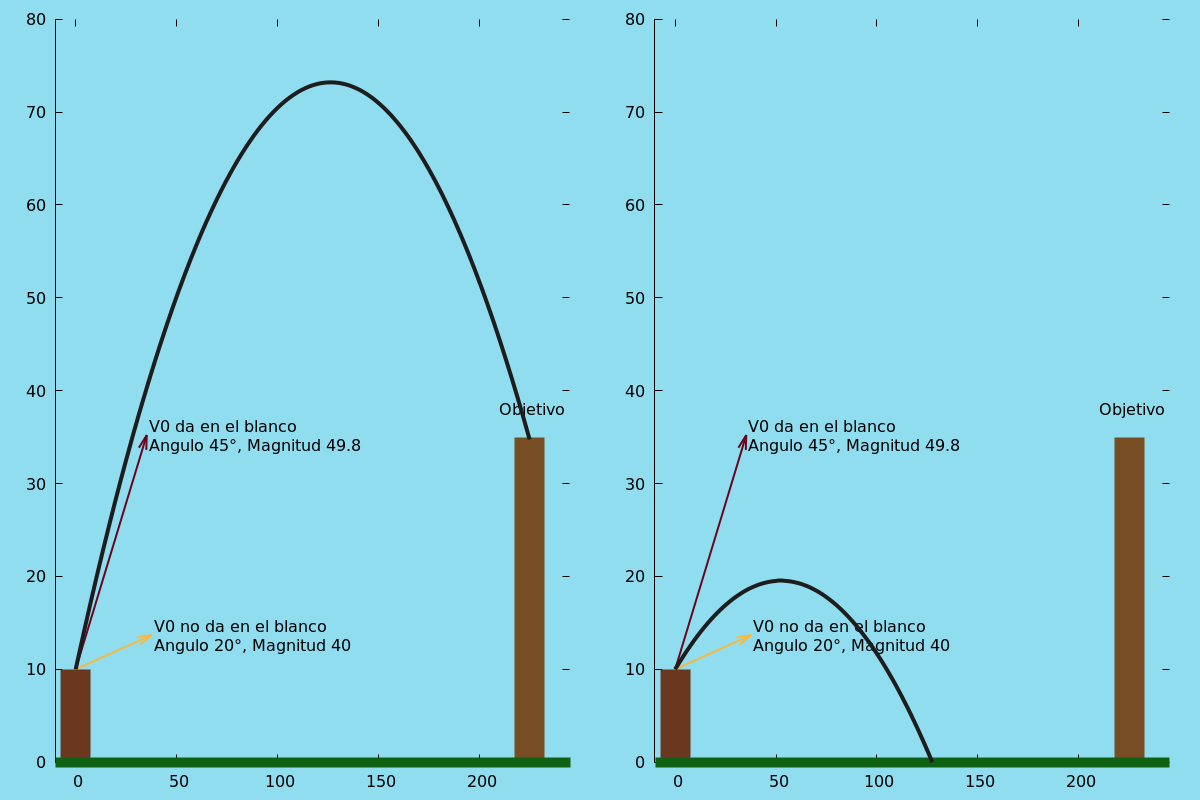
\includegraphics[scale=0.35]{images/trayectorias.png}
        \caption{Gráfica de trayectorias semiparabolicas.}
        \label{img}
    \end{figure}

    El siguiente es el diagrama de flujo

    \begin{figure}[H]
        \centering
        \includegraphics[scale=0.35]{images/diagrama.png}
        \caption{Diagrama de flujo.}
        \label{img}
    \end{figure}

    \section{Animación tiró parabolico.}
    \subsection*{D.}
    Al no tener un orden realmente consecutivo, la animación generada presenta en algunos momentos saltos entre imágenes generadas para diferentes momentos de la trayectoria.

    La diferencia entre el uso del \texttt{setw} u otros métodos para mantener la misma longitud de los textos radica en que una de las animaciones podrá tener saltos temporales durante la duración esta, mientras la que tenga estandarizada la longitud del texto mantendrá una misma secuencia.

    \subsection*{E.}
    La diferencia entre usar o no el comando \texttt{transparent} está en que al usarlo la superposición de las imágenes permite que las anteriores imágenes se visualicen, mientras que al no usarlo solo se ve la última de las imágenes.

    
    
    \section{Pregunta.}
    Si lo que se desea es no únicamente cambiar el nombre de la imagen que se va a generar, sino que también crear un archivo \texttt{.plt} especifico para cada una, lo que se requiere es modificar también el nombre de archivo que se le pasa al \texttt{ofstream} creado.
    
    Este cambio se puede realizar modificando el \texttt{string} que se le pasa como parámetro al método \texttt{open} con lo cual se reutiliza el ciclo \texttt{for} que se planteó anteriormente, pero en vez de cambiar únicamente el nombre de la imagen, también cambiar el nombre del archivo. 
    
    Hay que tener en cuenta que para cambiar el nombre que es de tipo \texttt{string} se utiliza el identificador que es de tipo \texttt{int} por lo que es necesario convertir el identificador a texto, lo cual exige usar la función \texttt{to\_string} pero antes realizar el \texttt{\#include <string>}.
\end{document}